\section{Results}
\label{sec:ch7-results}

\definecolor{ch7gain}{RGB}{0,110,55}
\definecolor{ch7loss}{RGB}{180,0,0}
\newcommand{\rgain}[1]{%
    \ifdim #1 pt < 0pt
        \textcolor{ch7loss}{#1}%
    \else
        \textcolor{ch7gain}{+#1}%
    \fi
}
\newcommand{\pns}[1]{#1 (n.s.)}

Each of the following subsections reports the results of one model. Its table reports, for the single-turn and the multi-turn dataset separately, the following data:

\begin{itemize}
    \item the optimal layer found by the layer sweep;
    \item the AUC macro of the probe at that layer;
    \item the model accuracy, on the whole dataset and on the \texttt{adversarial} tier alone;
    \item the probe accuracy at the optimal layer, on the whole dataset and on the \texttt{adversarial} tier alone;
    \item the difference $\Delta$ between probe accuracy and model accuracy, on the whole dataset and on the \texttt{adversarial} tier alone;
    \item the $p_{\text{holm}}$ of the McNemar test on $\Delta$, on the whole dataset and on the \texttt{adversarial} tier alone, corrected across all the tests of this section.
\end{itemize}

In every table, a $\Delta$ in \textcolor{ch7gain}{green} marks a probe more accurate than the model, and a $\Delta$ in \textcolor{ch7loss}{red} marks a probe less accurate than the model. A $p_{\text{holm}}$ followed by (n.s.) is a difference that is not significant at the 0.05 threshold.

A plot then compares the accuracy of the model, the probe and the text-only classifiers of Section~\ref{subsec:text-only-baselines}, on the whole dataset and on each difficulty tier. For each accuracy, an interval marks the lowest and the highest accuracy obtained on a held-out fold. The layer sweeps are reported in Appendix~\ref{chap:appendix-layer-sweeps}.

\subsection{Gemma 4 E2B IT}
\label{subsec:ch7-gemma4-e2b-it}

\begin{table}[H]
    \centering
    \small
    \setlength{\tabcolsep}{3.5pt}
    \begin{tabular}{@{}lcccccccccc@{}}
        \toprule
        & & & \multicolumn{4}{c}{\textbf{all}} & \multicolumn{4}{c}{\textbf{adversarial}} \\
        \cmidrule(lr){4-7} \cmidrule(lr){8-11}
        & \textbf{optimal layer} & \textbf{AUC macro} & \textbf{model} & \textbf{probe} & $\boldsymbol{\Delta}$ & $\boldsymbol{p_{\text{holm}}}$ & \textbf{model} & \textbf{probe} & $\boldsymbol{\Delta}$ & $\boldsymbol{p_{\text{holm}}}$ \\
        \midrule
        Single-turn & 22/35 & 0.976 & 0.736 & 0.848 & \rgain{0.112} & $<10^{-4}$ & 0.616 & 0.784 & \rgain{0.168} & $<10^{-4}$ \\
        Multi-turn & 17/35 & 0.947 & 0.702 & 0.782 & \rgain{0.080} & $<10^{-4}$ & 0.541 & 0.689 & \rgain{0.148} & $<10^{-4}$ \\
        \bottomrule
    \end{tabular}
    \caption[\texttt{gemma4-e2b-it}, probe against model, both datasets]{\texttt{gemma4-e2b-it}, probe against model, both datasets.}
    \label{tab:ch7-gemma4-e2b-it}
\end{table}

\begin{figure}[H]
    \centering
    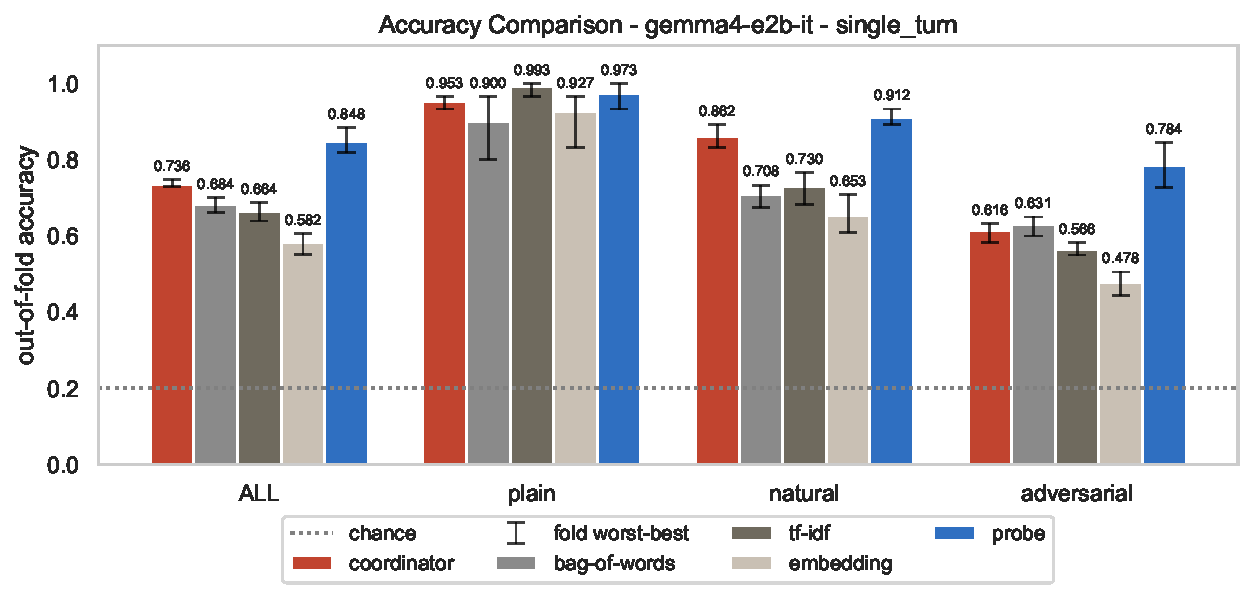
\includegraphics[width=0.85\textwidth]{images/models/gemma4-e2b-it_single_turn_routers.pdf}
    \caption[Accuracy comparison, gemma4-e2b-it, single-turn]{Accuracy comparison, gemma4-e2b-it, single-turn.}
    \label{fig:ch7-gemma4-e2b-it-single-routers}
\end{figure}

\begin{figure}[H]
    \centering
    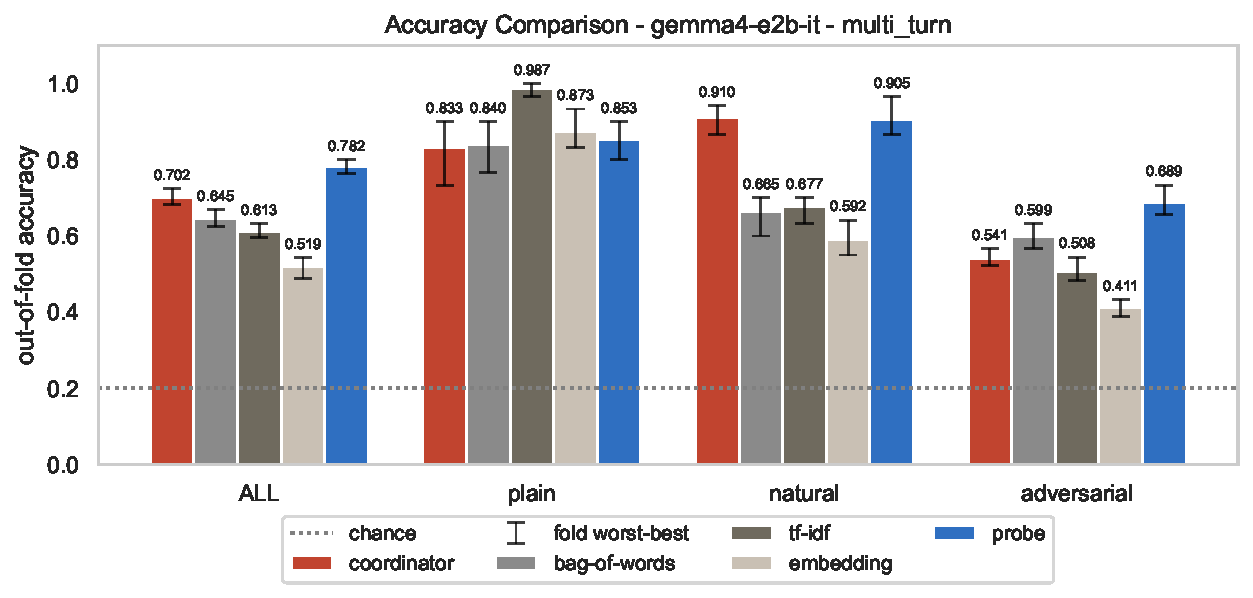
\includegraphics[width=0.85\textwidth]{images/models/gemma4-e2b-it_multi_turn_routers.pdf}
    \caption[Accuracy comparison, gemma4-e2b-it, multi-turn]{Accuracy comparison, gemma4-e2b-it, multi-turn.}
    \label{fig:ch7-gemma4-e2b-it-multi-routers}
\end{figure}


\clearpage

\subsection{Qwen3 4B Instruct 2507}
\label{subsec:ch7-qwen3-4b}

\begin{table}[H]
    \centering
    \small
    \setlength{\tabcolsep}{3.5pt}
    \begin{tabular}{@{}lcccccccccc@{}}
        \toprule
        & & & \multicolumn{4}{c}{\textbf{all}} & \multicolumn{4}{c}{\textbf{adversarial}} \\
        \cmidrule(lr){4-7} \cmidrule(lr){8-11}
        & \textbf{optimal layer} & \textbf{AUC macro} & \textbf{model} & \textbf{probe} & $\boldsymbol{\Delta}$ & $\boldsymbol{p_{\text{holm}}}$ & \textbf{model} & \textbf{probe} & $\boldsymbol{\Delta}$ & $\boldsymbol{p_{\text{holm}}}$ \\
        \midrule
        Single-turn & 23/36 & 0.977 & 0.752 & 0.864 & \rgain{0.112} & $<10^{-4}$ & 0.610 & 0.806 & \rgain{0.196} & $<10^{-4}$ \\
        Multi-turn & 23/36 & 0.959 & 0.745 & 0.814 & \rgain{0.069} & $<10^{-4}$ & 0.602 & 0.718 & \rgain{0.116} & $<10^{-4}$ \\
        \bottomrule
    \end{tabular}
    \caption[\texttt{qwen3-4b}, probe against model, both datasets]{\texttt{qwen3-4b}, probe against model, both datasets.}
    \label{tab:ch7-qwen3-4b}
\end{table}

\begin{figure}[H]
    \centering
    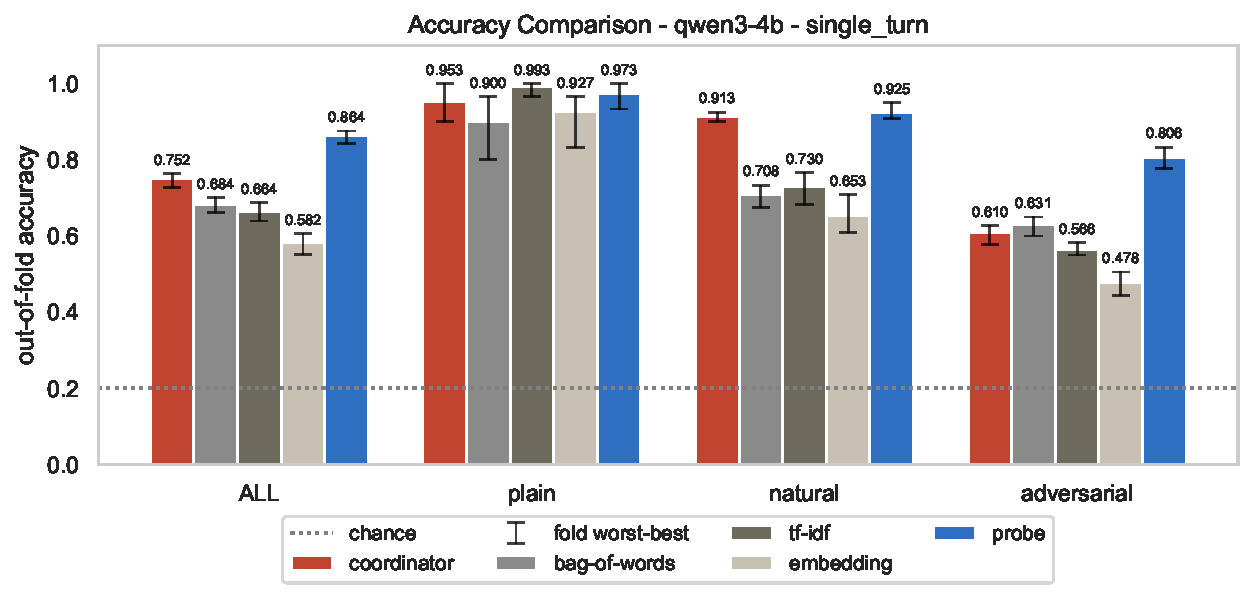
\includegraphics[width=0.85\textwidth]{images/models/qwen3-4b_single_turn_routers.pdf}
    \caption[Accuracy comparison, qwen3-4b, single-turn]{Accuracy comparison, qwen3-4b, single-turn.}
    \label{fig:ch7-qwen3-4b-single-routers}
\end{figure}

\begin{figure}[H]
    \centering
    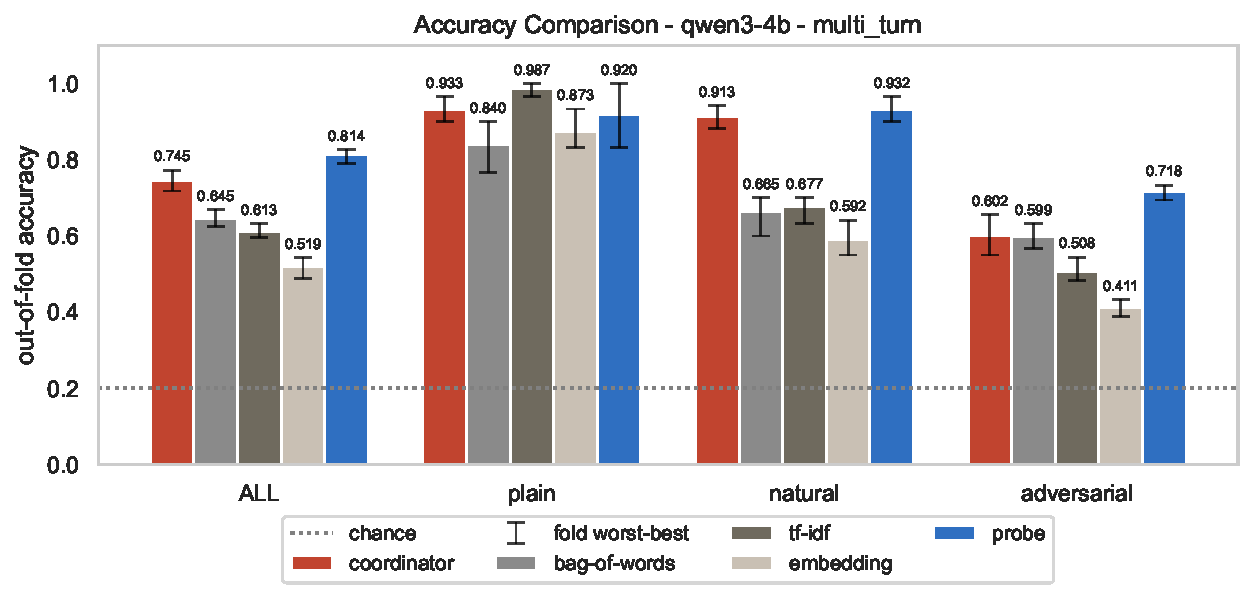
\includegraphics[width=0.85\textwidth]{images/models/qwen3-4b_multi_turn_routers.pdf}
    \caption[Accuracy comparison, qwen3-4b, multi-turn]{Accuracy comparison, qwen3-4b, multi-turn.}
    \label{fig:ch7-qwen3-4b-multi-routers}
\end{figure}


\clearpage

\subsection{Qwen3 8B}
\label{subsec:ch7-qwen3-8b}

\begin{table}[H]
    \centering
    \small
    \setlength{\tabcolsep}{3.5pt}
    \begin{tabular}{@{}lcccccccccc@{}}
        \toprule
        & & & \multicolumn{4}{c}{\textbf{all}} & \multicolumn{4}{c}{\textbf{adversarial}} \\
        \cmidrule(lr){4-7} \cmidrule(lr){8-11}
        & \textbf{optimal layer} & \textbf{AUC macro} & \textbf{model} & \textbf{probe} & $\boldsymbol{\Delta}$ & $\boldsymbol{p_{\text{holm}}}$ & \textbf{model} & \textbf{probe} & $\boldsymbol{\Delta}$ & $\boldsymbol{p_{\text{holm}}}$ \\
        \midrule
        Single-turn & 23/36 & 0.974 & 0.772 & 0.845 & \rgain{0.073} & $<10^{-4}$ & 0.652 & 0.784 & \rgain{0.132} & $<10^{-4}$ \\
        Multi-turn & 30/36 & 0.928 & 0.738 & 0.744 & \rgain{0.006} & \pns{0.65} & 0.597 & 0.634 & \rgain{0.037} & \pns{0.10} \\
        \bottomrule
    \end{tabular}
    \caption[\texttt{qwen3-8b}, probe against model, both datasets]{\texttt{qwen3-8b}, probe against model, both datasets.}
    \label{tab:ch7-qwen3-8b}
\end{table}

\begin{figure}[H]
    \centering
    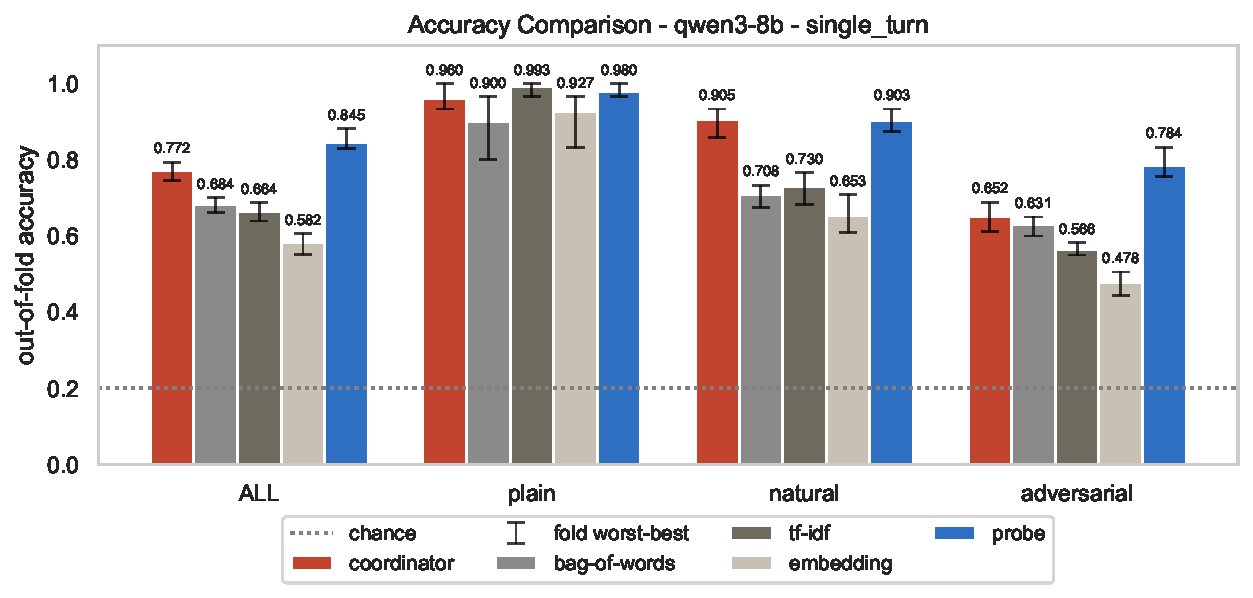
\includegraphics[width=0.85\textwidth]{images/models/qwen3-8b_single_turn_routers.pdf}
    \caption[Accuracy comparison, qwen3-8b, single-turn]{Accuracy comparison, qwen3-8b, single-turn.}
    \label{fig:ch7-qwen3-8b-single-routers}
\end{figure}

\begin{figure}[H]
    \centering
    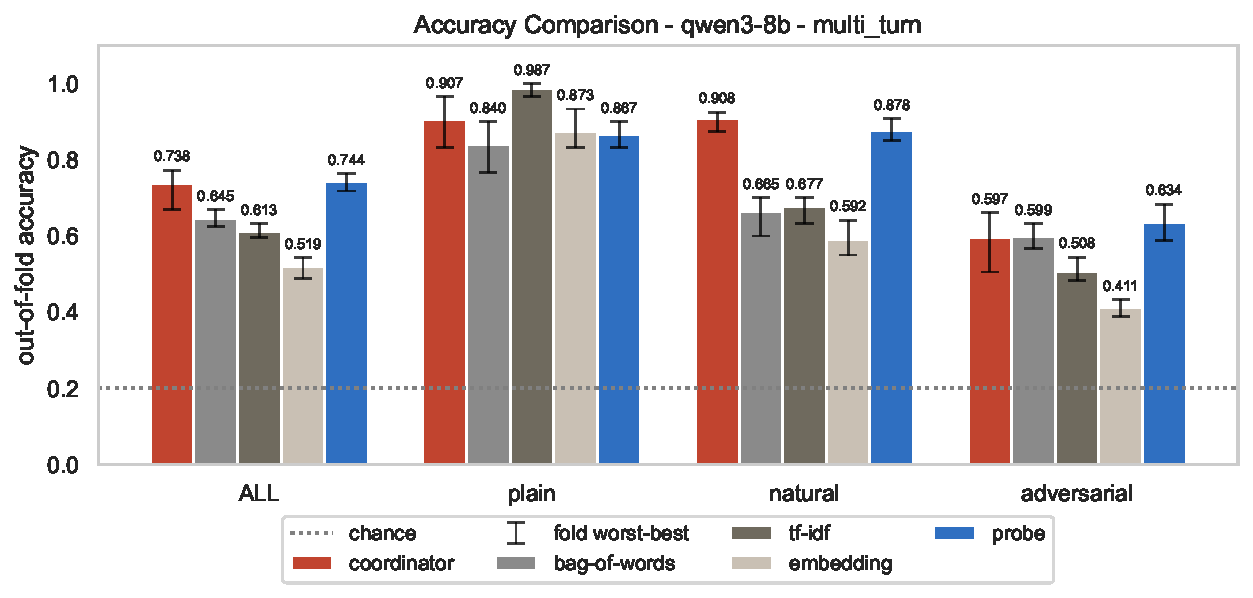
\includegraphics[width=0.85\textwidth]{images/models/qwen3-8b_multi_turn_routers.pdf}
    \caption[Accuracy comparison, qwen3-8b, multi-turn]{Accuracy comparison, qwen3-8b, multi-turn.}
    \label{fig:ch7-qwen3-8b-multi-routers}
\end{figure}


\clearpage

\subsection{Gemma 4 12B IT}
\label{subsec:ch7-gemma4-12b-it}

\begin{table}[H]
    \centering
    \small
    \setlength{\tabcolsep}{3.5pt}
    \begin{tabular}{@{}lcccccccccc@{}}
        \toprule
        & & & \multicolumn{4}{c}{\textbf{all}} & \multicolumn{4}{c}{\textbf{adversarial}} \\
        \cmidrule(lr){4-7} \cmidrule(lr){8-11}
        & \textbf{optimal layer} & \textbf{AUC macro} & \textbf{model} & \textbf{probe} & $\boldsymbol{\Delta}$ & $\boldsymbol{p_{\text{holm}}}$ & \textbf{model} & \textbf{probe} & $\boldsymbol{\Delta}$ & $\boldsymbol{p_{\text{holm}}}$ \\
        \midrule
        Single-turn & 31/48 & 0.988 & 0.873 & 0.916 & \rgain{0.043} & $<10^{-4}$ & 0.829 & 0.884 & \rgain{0.055} & $<10^{-4}$ \\
        Multi-turn & 32/48 & 0.979 & 0.855 & 0.879 & \rgain{0.024} & 0.011 & 0.777 & 0.827 & \rgain{0.050} & 0.00048 \\
        \bottomrule
    \end{tabular}
    \caption[\texttt{gemma4-12b-it}, probe against model, both datasets]{\texttt{gemma4-12b-it}, probe against model, both datasets.}
    \label{tab:ch7-gemma4-12b-it}
\end{table}

\begin{figure}[H]
    \centering
    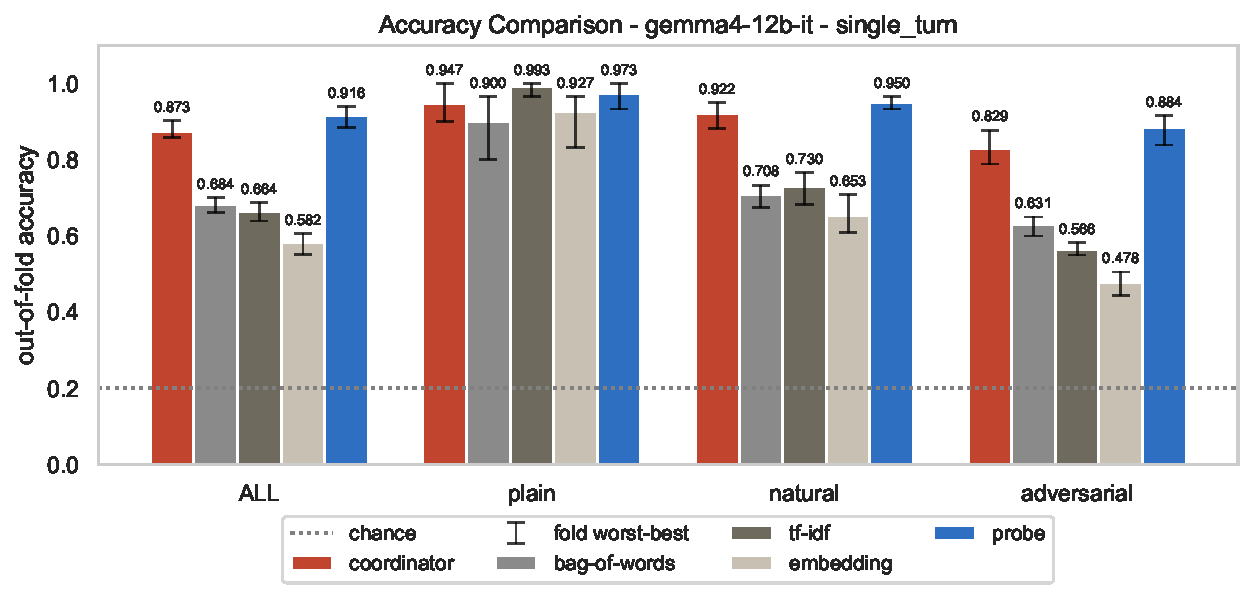
\includegraphics[width=0.85\textwidth]{images/models/gemma4-12b-it_single_turn_routers.pdf}
    \caption[Accuracy comparison, gemma4-12b-it, single-turn]{Accuracy comparison, gemma4-12b-it, single-turn.}
    \label{fig:ch7-gemma4-12b-it-single-routers}
\end{figure}

\begin{figure}[H]
    \centering
    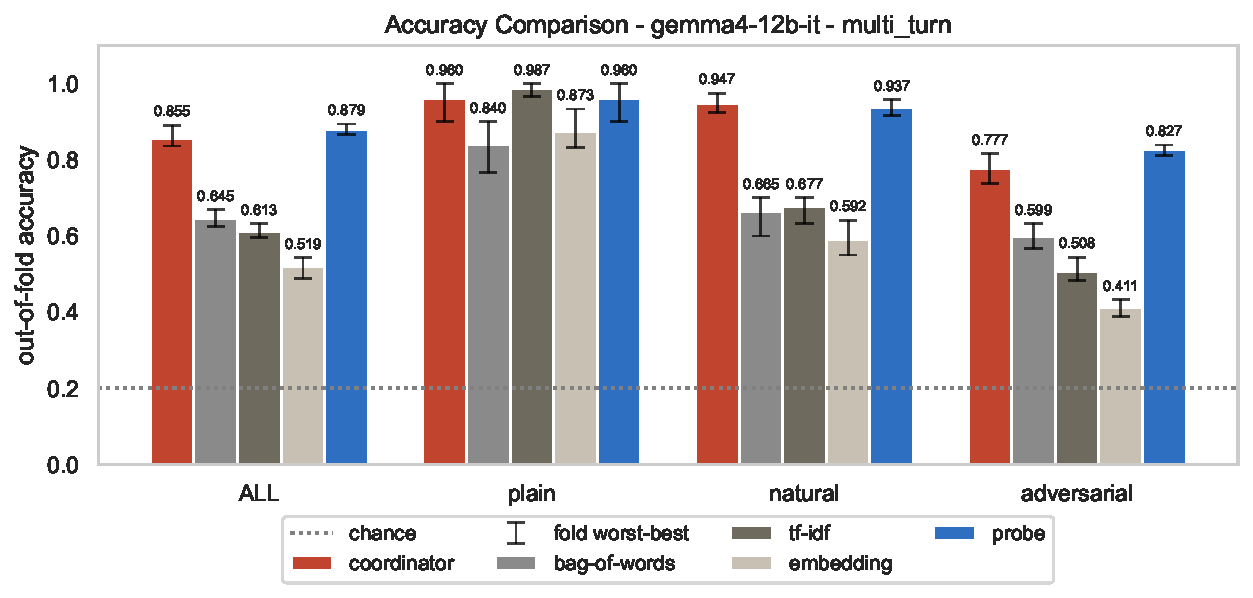
\includegraphics[width=0.85\textwidth]{images/models/gemma4-12b-it_multi_turn_routers.pdf}
    \caption[Accuracy comparison, gemma4-12b-it, multi-turn]{Accuracy comparison, gemma4-12b-it, multi-turn.}
    \label{fig:ch7-gemma4-12b-it-multi-routers}
\end{figure}


\clearpage

\subsection{GPT-OSS 20B}
\label{subsec:ch7-gpt-oss-20b}

\begin{table}[H]
    \centering
    \small
    \setlength{\tabcolsep}{3.5pt}
    \begin{tabular}{@{}lcccccccccc@{}}
        \toprule
        & & & \multicolumn{4}{c}{\textbf{all}} & \multicolumn{4}{c}{\textbf{adversarial}} \\
        \cmidrule(lr){4-7} \cmidrule(lr){8-11}
        & \textbf{optimal layer} & \textbf{AUC macro} & \textbf{model} & \textbf{probe} & $\boldsymbol{\Delta}$ & $\boldsymbol{p_{\text{holm}}}$ & \textbf{model} & \textbf{probe} & $\boldsymbol{\Delta}$ & $\boldsymbol{p_{\text{holm}}}$ \\
        \midrule
        Single-turn & 18/24 & 0.915 & 0.818 & 0.689 & \rgain{-0.129} & $<10^{-4}$ & 0.737 & 0.601 & \rgain{-0.136} & $<10^{-4}$ \\
        Multi-turn & 18/24 & 0.788 & 0.719 & 0.505 & \rgain{-0.214} & $<10^{-4}$ & 0.607 & 0.438 & \rgain{-0.169} & $<10^{-4}$ \\
        \bottomrule
    \end{tabular}
    \caption[\texttt{gpt-oss-20b}, probe against model, both datasets]{\texttt{gpt-oss-20b}, probe against model, both datasets.}
    \label{tab:ch7-gpt-oss-20b}
\end{table}

\begin{figure}[H]
    \centering
    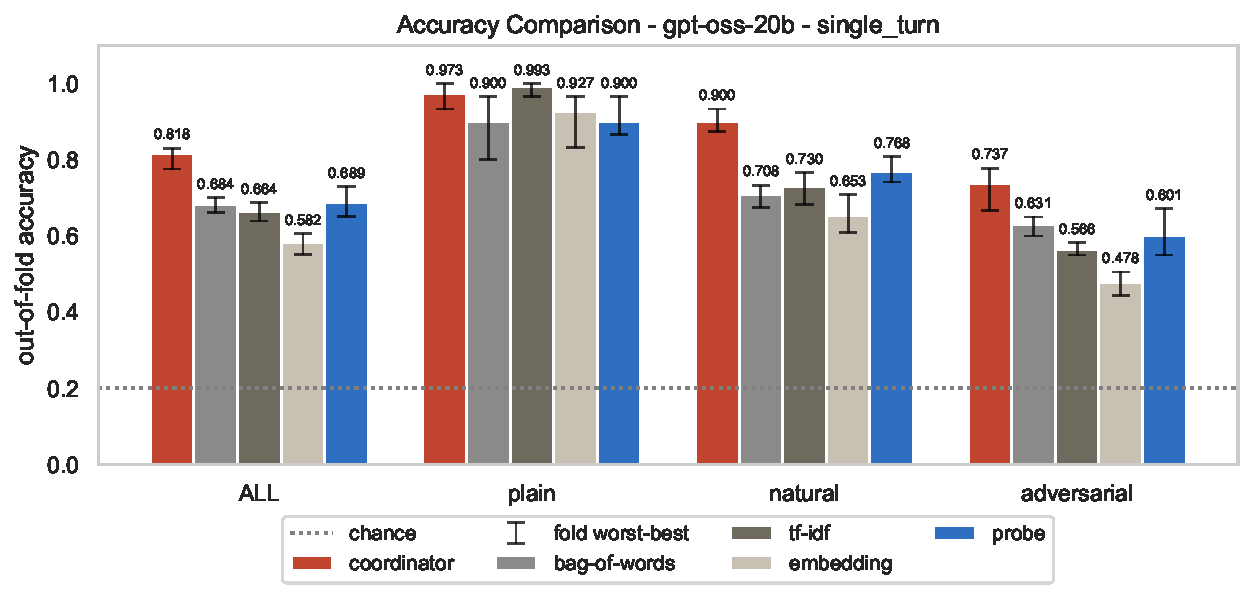
\includegraphics[width=0.85\textwidth]{images/models/gpt-oss-20b_single_turn_routers.pdf}
    \caption[Accuracy comparison, gpt-oss-20b, single-turn]{Accuracy comparison, gpt-oss-20b, single-turn.}
    \label{fig:ch7-gpt-oss-20b-single-routers}
\end{figure}

\begin{figure}[H]
    \centering
    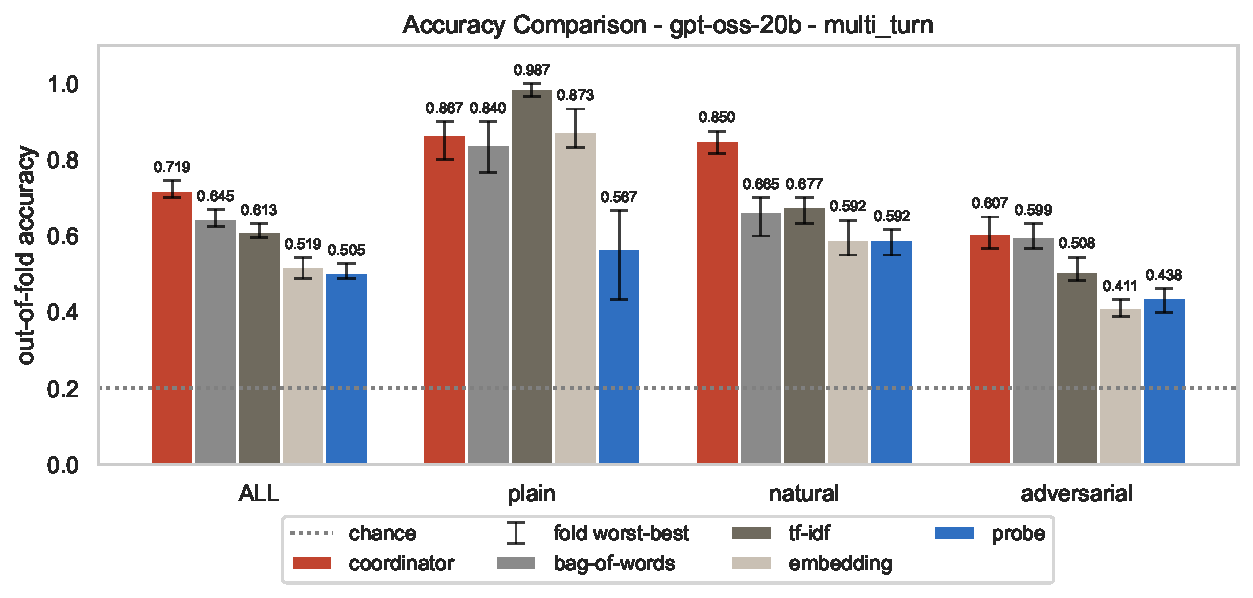
\includegraphics[width=0.85\textwidth]{images/models/gpt-oss-20b_multi_turn_routers.pdf}
    \caption[Accuracy comparison, gpt-oss-20b, multi-turn]{Accuracy comparison, gpt-oss-20b, multi-turn.}
    \label{fig:ch7-gpt-oss-20b-multi-routers}
\end{figure}


\clearpage

\subsection{Gemma 4 26B A4B IT}
\label{subsec:ch7-gemma4-26b-a4b-it}

\begin{table}[H]
    \centering
    \small
    \setlength{\tabcolsep}{3.5pt}
    \begin{tabular}{@{}lcccccccccc@{}}
        \toprule
        & & & \multicolumn{4}{c}{\textbf{all}} & \multicolumn{4}{c}{\textbf{adversarial}} \\
        \cmidrule(lr){4-7} \cmidrule(lr){8-11}
        & \textbf{optimal layer} & \textbf{AUC macro} & \textbf{model} & \textbf{probe} & $\boldsymbol{\Delta}$ & $\boldsymbol{p_{\text{holm}}}$ & \textbf{model} & \textbf{probe} & $\boldsymbol{\Delta}$ & $\boldsymbol{p_{\text{holm}}}$ \\
        \midrule
        Single-turn & 19/30 & 0.989 & 0.888 & 0.921 & \rgain{0.033} & 0.00012 & 0.841 & 0.888 & \rgain{0.047} & 0.001 \\
        Multi-turn & 19/30 & 0.977 & 0.856 & 0.878 & \rgain{0.022} & 0.024 & 0.773 & 0.831 & \rgain{0.058} & 0.00016 \\
        \bottomrule
    \end{tabular}
    \caption[\texttt{gemma4-26b-a4b-it}, probe against model, both datasets]{\texttt{gemma4-26b-a4b-it}, probe against model, both datasets.}
    \label{tab:ch7-gemma4-26b-a4b-it}
\end{table}

\begin{figure}[H]
    \centering
    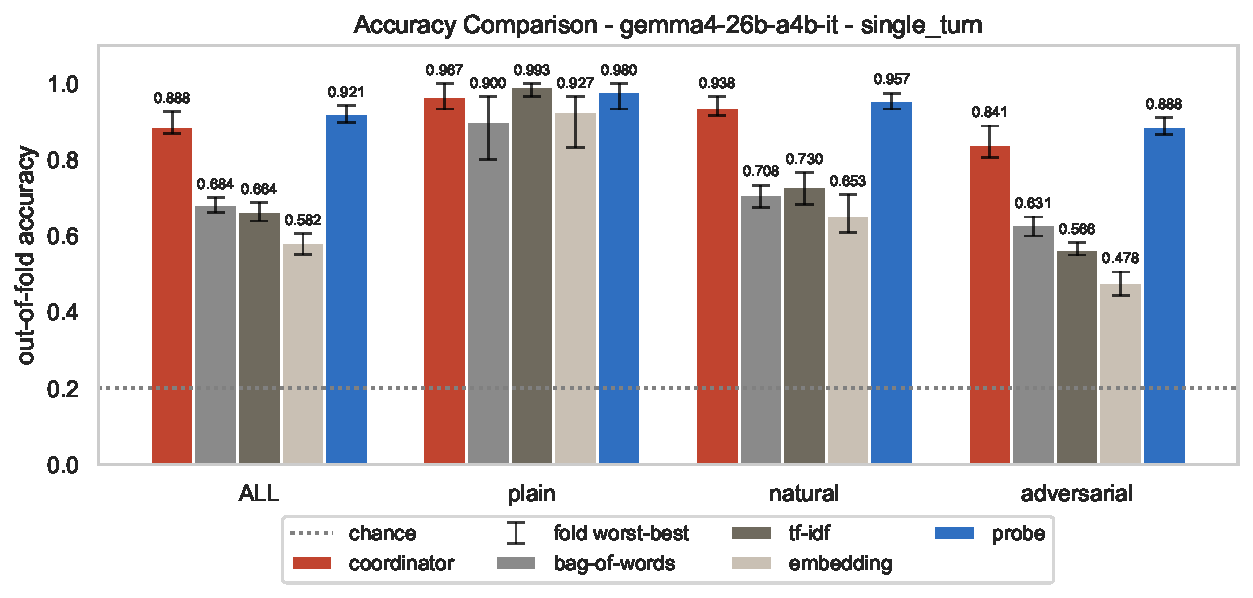
\includegraphics[width=0.85\textwidth]{images/models/gemma4-26b-a4b-it_single_turn_routers.pdf}
    \caption[Accuracy comparison, gemma4-26b-a4b-it, single-turn]{Accuracy comparison, gemma4-26b-a4b-it, single-turn.}
    \label{fig:ch7-gemma4-26b-a4b-it-single-routers}
\end{figure}

\begin{figure}[H]
    \centering
    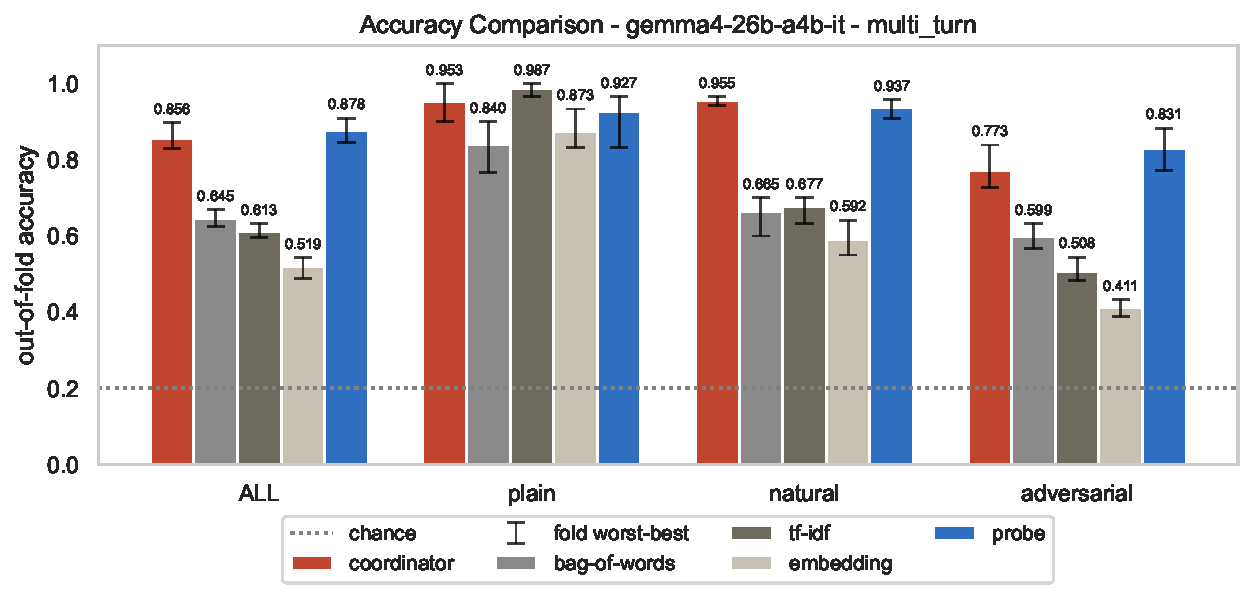
\includegraphics[width=0.85\textwidth]{images/models/gemma4-26b-a4b-it_multi_turn_routers.pdf}
    \caption[Accuracy comparison, gemma4-26b-a4b-it, multi-turn]{Accuracy comparison, gemma4-26b-a4b-it, multi-turn.}
    \label{fig:ch7-gemma4-26b-a4b-it-multi-routers}
\end{figure}


\clearpage

\subsection{Llama 3.3 70B Instruct}
\label{subsec:ch7-llama33-70b}

\begin{table}[H]
    \centering
    \small
    \setlength{\tabcolsep}{3.5pt}
    \begin{tabular}{@{}lcccccccccc@{}}
        \toprule
        & & & \multicolumn{4}{c}{\textbf{all}} & \multicolumn{4}{c}{\textbf{adversarial}} \\
        \cmidrule(lr){4-7} \cmidrule(lr){8-11}
        & \textbf{optimal layer} & \textbf{AUC macro} & \textbf{model} & \textbf{probe} & $\boldsymbol{\Delta}$ & $\boldsymbol{p_{\text{holm}}}$ & \textbf{model} & \textbf{probe} & $\boldsymbol{\Delta}$ & $\boldsymbol{p_{\text{holm}}}$ \\
        \midrule
        Single-turn & 42/80 & 0.985 & 0.770 & 0.894 & \rgain{0.124} & $<10^{-4}$ & 0.667 & 0.847 & \rgain{0.180} & $<10^{-4}$ \\
        Multi-turn & 38/80 & 0.950 & 0.736 & 0.810 & \rgain{0.074} & $<10^{-4}$ & 0.606 & 0.714 & \rgain{0.108} & $<10^{-4}$ \\
        \bottomrule
    \end{tabular}
    \caption[\texttt{llama3.3-70b}, probe against model, both datasets]{\texttt{llama3.3-70b}, probe against model, both datasets.}
    \label{tab:ch7-llama33-70b}
\end{table}

\begin{figure}[H]
    \centering
    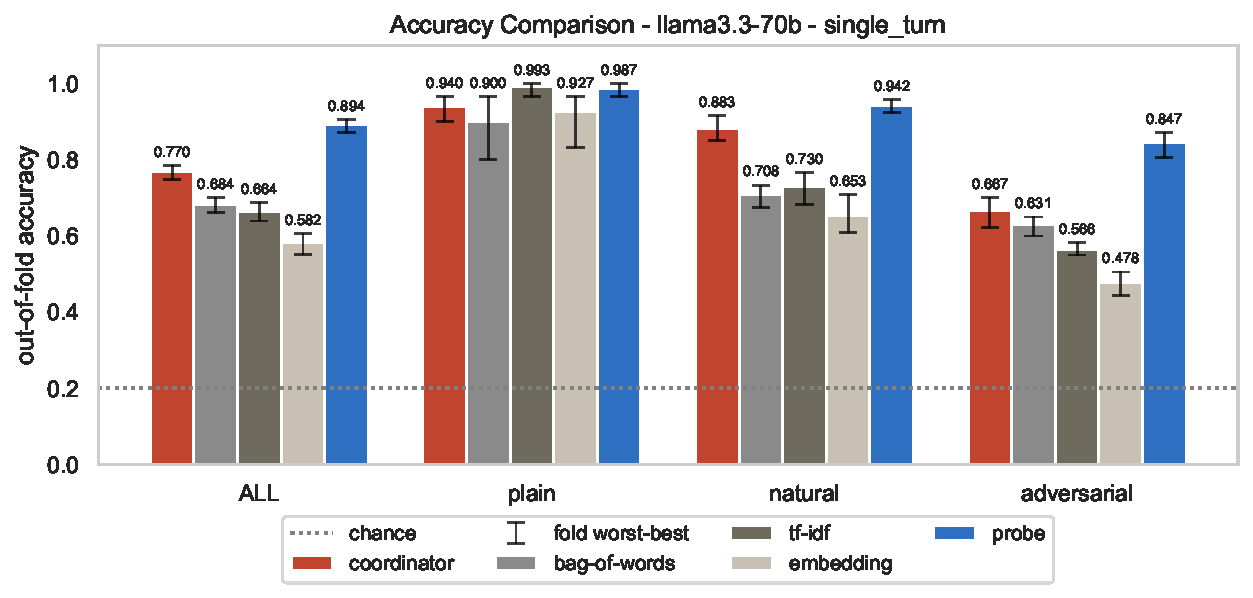
\includegraphics[width=0.85\textwidth]{images/models/llama33-70b_single_turn_routers.pdf}
    \caption[Accuracy comparison, llama3.3-70b, single-turn]{Accuracy comparison, llama3.3-70b, single-turn.}
    \label{fig:ch7-llama33-70b-single-routers}
\end{figure}

\begin{figure}[H]
    \centering
    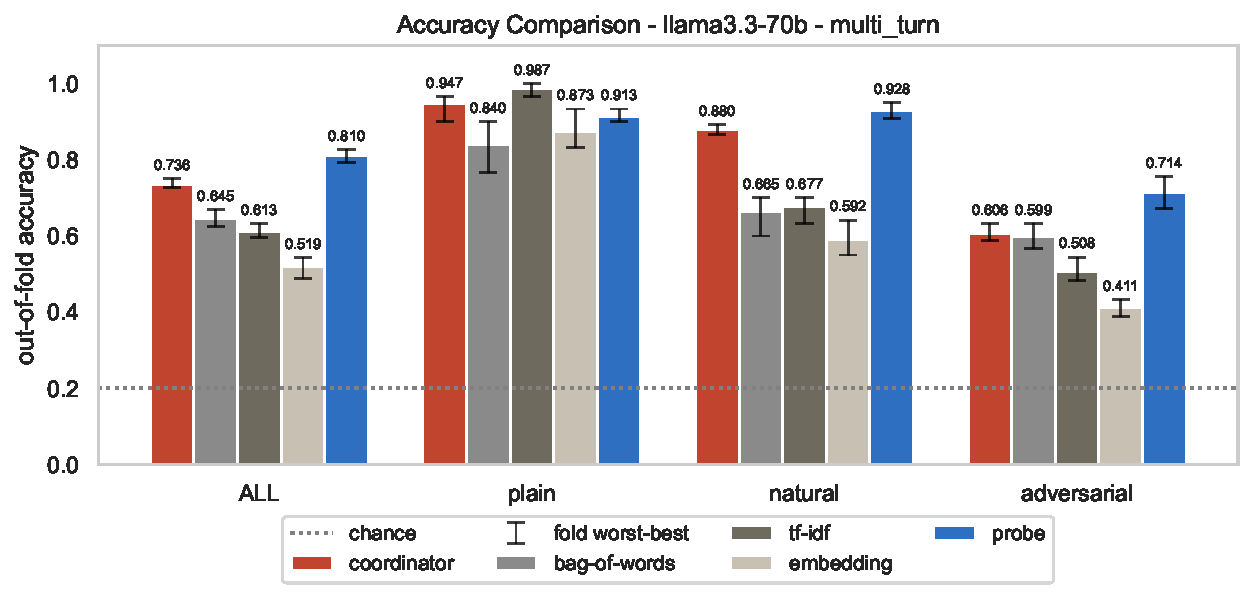
\includegraphics[width=0.85\textwidth]{images/models/llama33-70b_multi_turn_routers.pdf}
    \caption[Accuracy comparison, llama3.3-70b, multi-turn]{Accuracy comparison, llama3.3-70b, multi-turn.}
    \label{fig:ch7-llama33-70b-multi-routers}
\end{figure}


\clearpage

\subsection{Qwen2.5 72B Instruct}
\label{subsec:ch7-qwen25-72b}

\begin{table}[H]
    \centering
    \small
    \setlength{\tabcolsep}{3.5pt}
    \begin{tabular}{@{}lcccccccccc@{}}
        \toprule
        & & & \multicolumn{4}{c}{\textbf{all}} & \multicolumn{4}{c}{\textbf{adversarial}} \\
        \cmidrule(lr){4-7} \cmidrule(lr){8-11}
        & \textbf{optimal layer} & \textbf{AUC macro} & \textbf{model} & \textbf{probe} & $\boldsymbol{\Delta}$ & $\boldsymbol{p_{\text{holm}}}$ & \textbf{model} & \textbf{probe} & $\boldsymbol{\Delta}$ & $\boldsymbol{p_{\text{holm}}}$ \\
        \midrule
        Single-turn & 55/80 & 0.988 & 0.761 & 0.907 & \rgain{0.146} & $<10^{-4}$ & 0.638 & 0.862 & \rgain{0.224} & $<10^{-4}$ \\
        Multi-turn & 58/80 & 0.976 & 0.768 & 0.875 & \rgain{0.107} & $<10^{-4}$ & 0.629 & 0.800 & \rgain{0.171} & $<10^{-4}$ \\
        \bottomrule
    \end{tabular}
    \caption[\texttt{qwen2.5-72b}, probe against model, both datasets]{\texttt{qwen2.5-72b}, probe against model, both datasets.}
    \label{tab:ch7-qwen25-72b}
\end{table}

\begin{figure}[H]
    \centering
    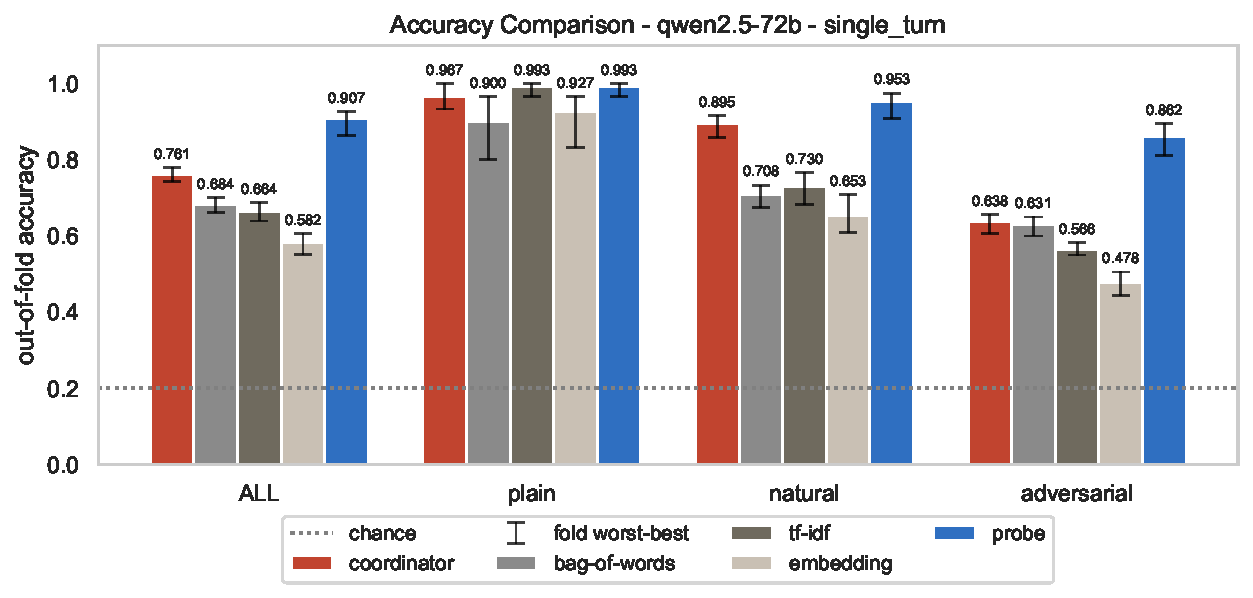
\includegraphics[width=0.85\textwidth]{images/models/qwen25-72b_single_turn_routers.pdf}
    \caption[Accuracy comparison, qwen2.5-72b, single-turn]{Accuracy comparison, qwen2.5-72b, single-turn.}
    \label{fig:ch7-qwen25-72b-single-routers}
\end{figure}

\begin{figure}[H]
    \centering
    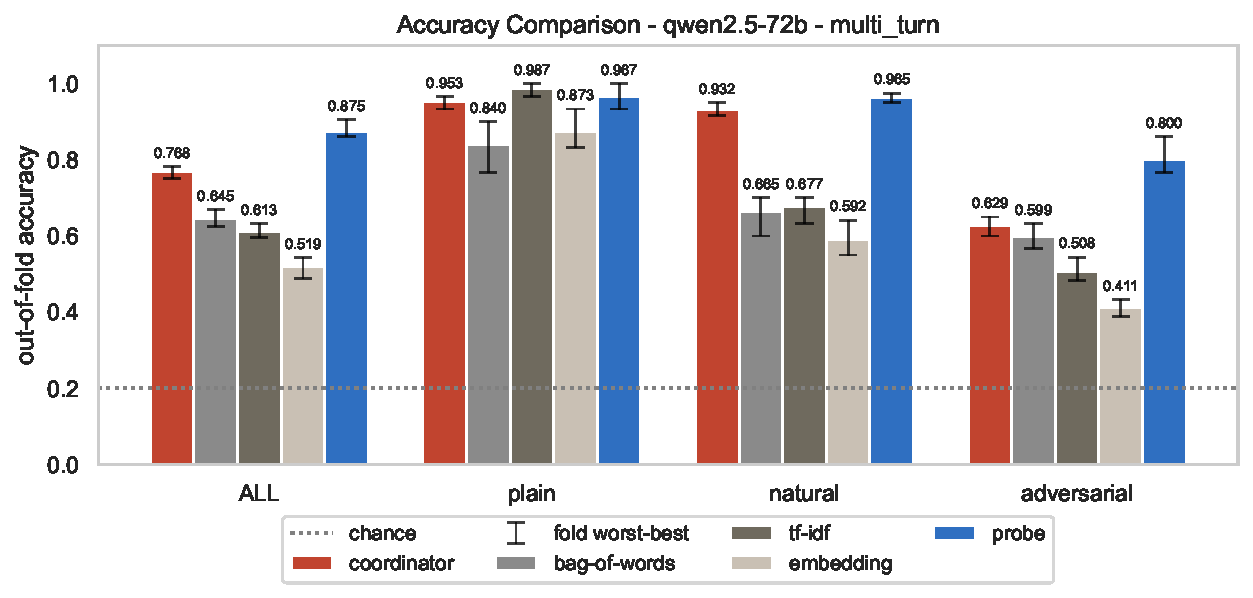
\includegraphics[width=0.85\textwidth]{images/models/qwen25-72b_multi_turn_routers.pdf}
    \caption[Accuracy comparison, qwen2.5-72b, multi-turn]{Accuracy comparison, qwen2.5-72b, multi-turn.}
    \label{fig:ch7-qwen25-72b-multi-routers}
\end{figure}

